%!TEX TS-program = xelatex
%-=-=-=-=-=-=-=-=-=-=-=-=-=-=-=-=-=-=-=-=-=-=-=-=
% Deedy - One Page Two Column Resume
% LaTeX Template
% Version 1.2 (16/9/2014)
%
% Original author:
% Debarghya Das (http://debarghyadas.com)
%
% Original repository:
% https://github.com/deedydas/Deedy-Resume
%
% IMPORTANT: THIS TEMPLATE NEEDS TO BE COMPILED WITH XeLaTeX
%
% This template uses several fonts not included with Windows/Linux by
% default. If you get compilation errors saying a font is missing, find the line
% on which the font is used and either change it to a font included with your
% operating system or comment the line out to use the default font.
% 
%
% CHANGELOG:
% v1.1:
% 1. Fixed several compilation bugs with \renewcommand
% 2. Got Open-source fonts (Windows/Linux support)
% 3. Added Last Updated
% 4. Move Title styling into .sty
% 5. Commented .sty file.
%
%-=-=-=-=-=-=-=-=-=-=-=-=-=-=-=-=-=-=-=-=-=-=-=-=
%
% Known Issues:
% 1. Overflows onto second page if any column's contents are more than the
% vertical limit
% 2. Hacky space on the first bullet point on the second column.
%
%-=-=-=-=-=-=-=-=-=-=-=-=-=-=-=-=-=-=-=


\documentclass[a4paper]{deedy-resume}
\usepackage{fancyhdr}
\usepackage{multicol}
\usepackage{smartdiagram}
%\graphicspath{{\string~/Documents/latex/assets/}} 
\pagestyle{fancy}
\fancyhf{}
 
\rfoot{Page \thepage \hspace{1pt}}

%-=-=-=-=-=-=-=-=-=-=-=-=-=-=-=-=-=-=-=-=-=-=-=-=
%   My Customizatins  =-=-=-=-=-=-=-=-=-=-=-=-=-=

% CUSTOM COLORS
\definecolor{cvblue}{RGB}{0,75,90} % HEX #fedeed
\newcommand{\cvblue}[1]{{\color{cvblue}{#1}}}
\newcommand{\ccvblue}{cvblue}
\newcommand{\crcvblue}{\color{cvblue}}
\newcommand{\doneit}{\small{\cvblue{$\odot$}}}
\newcommand{\itemit}{\cvblue{$\odot$ \,}}
\usepackage{xspace}
\newcommand{\TikZ}{Ti\textit{k}Z\xspace}

\usepackage{chronology}
\renewcommand{\event}[3][e]{%
  \pgfmathsetlength\xstop{(#2-\theyearstart)*\unit}%
  \ifx #1e%
    \draw[fill=black,draw=none,opacity=0.5]%
      (\xstop, 0) circle (.2\unit)%
      node[opacity=1,rotate=45,right=.2\unit] {#3};%
  \else%
    \pgfmathsetlength\xstart{(#1-\theyearstart)*\unit}%
    \draw[fill=black,draw=none,opacity=0.5,rounded corners=.1\unit]%
      (\xstart,-.1\unit) rectangle%
      node[opacity=1,rotate=45,right=.2\unit] {#3} (\xstop,.1\unit);%
  \fi}%
\newcommand{\cevent}[3][e]{%
  \pgfmathsetlength\xstop{(#2-\theyearstart)*\unit}%
  \ifx #1e%
    \draw[fill=\ccvblue,draw=none,opacity=0.5]%
      (\xstop, 0) circle (.2\unit)%
      node[opacity=1,rotate=45,right=.2\unit] {#3};%
  \else%
    \pgfmathsetlength\xstart{(#1-\theyearstart)*\unit}%
    \draw[fill=\ccvblue,draw=none,opacity=0.5,rounded corners=.1\unit]%
      (\xstart,-.1\unit) rectangle%
      node[opacity=1,rotate=45,right=.2\unit] {#3} (\xstop,.1\unit);%
  \fi}%
%   Customizations END  =-=-=-=-=-=-=-=-=-=-=-=-=
%-=-=-=-=-=-=-=-=-=-=-=-=-=-=-=-=-=-=-=-=-=-=-=-=

\begin{document}

%-=-=-=-=-=-=-=-=-=-=-=-=-=-=-=-=-=-=-=
%
%     LAST UPDATED DATE
%
%-=-=-=-=-=-=-=-=-=-=-=-=-=-=-=-=-=-=-=
\lastupdated

%-=-=-=-=-=-=-=-=-=-=-=-=-=-=-=-=-=-=-=
%
%     TITLE NAME
%
%-=-=-=-=-=-=-=-=-=-=-=-=-=-=-=-=-=-=-=
\namesection{Mark Hendry}{\crcvblue{Olson}}{ \urlstyle{same}\href{http://markolson.se}{markolson.se} | +46 70 \#\#\# \#\#\#\# | \href{mailto:markolsonse@icloud.com}{markolsonse@icloud.com}  \\
Anothergatan 85 \#\#\# \#\# Stockholm
}

%-=-=-=-=-=-=-=-=-=-=-=-=-=-=-=-=-=-=-=
%
%     COLUMN ONE
%
%-=-=-=-=-=-=-=-=-=-=-=-=-=-=-=-=-=-=-=

\begin{minipage}[t]{0.33\textwidth} 
  
%-=-=-=-=-=-=-=-=-=-=-=-=-=-=-=-=-=-=-=
%     ABOUT
%-=-=-=-=-=-=-=-=-=-=-=-=-=-=-=-=-=-=-=

\section{About}

\includegraphics[width=0.9 \textwidth]{mho.jpg}\\

\itemit DOB: Jan 25 \\
\itemit Citizen of Canada \& Sweden \\
\itemit Run, Spin, Yoga \& Sauna 
\section{Technology}

\scalebox{0.6}{
\smartdiagramset{set color list={\ccvblue,\ccvblue,\ccvblue,\ccvblue,\ccvblue,\ccvblue,\ccvblue,},uniform connection color=true}

\smartdiagram[bubble diagram]{
Toolkit,Python \\ Matplotlib \\Sympy \\ Numpy,\LaTeX \\ \TikZ \\ Beamer  \\ Git, MacOS \\ ChromeOS \\ Linux, SchoolSoft \\ Managebac \\ Skola24 \\ Engage, TI84 \\ TI-Nspire \\ Casio CGFX-50, Google \\ Classroom \\ Colab}
}

\sectionsep
 
%-=-=-=-=-=-=-=-=-=-=-=-=-=-=-=-=-=-=-=
%     COURSES TAGHT
%-=-=-=-=-=-=-=-=-=-=-=-=-=-=-=-=-=-=-=
\section{Courses Taught}
\descript{Experience in years}
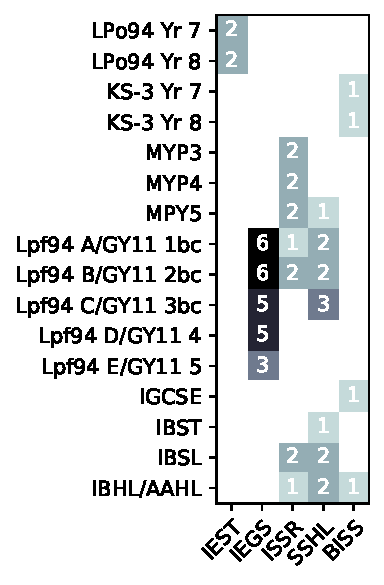
\includegraphics[width=0.9\textwidth]{cv-CoursesTaught}

%-=-=-=-=-=-=-=-=-=-=-=-=-=-=-=-=-=-=-=
%
%     COLUMN TWO
%
%-=-=-=-=-=-=-=-=-=-=-=-=-=-=-=-=-=-=-=

\end{minipage} 
\hfill
\begin{minipage}[t]{0.66\textwidth} 

%-=-=-=-=-=-=-=-=-=-=-=-=-=-=-=-=-=-=-=
%     EXPERIENCE
%-=-=-=-=-=-=-=-=-=-=-=-=-=-=-=-=-=-=-=

\section{Teaching Experience}
\begin{center}\begin{chronology}[2]{2005}{2020}{0.9\textwidth}
\event[\decimaldate{21}{7}{2005}]{\decimaldate{21}{7}{2006}}{Northern}
\event[\decimaldate{21}{7}{2006}]{\decimaldate{20}{7}{2008}}{IEST}
\event[\decimaldate{21}{7}{2008}]{\decimaldate{12}{8}{2014}}{IEGS}
\event[\decimaldate{13}{8}{2014}]{\decimaldate{16}{8}{2016}}{ISSR}
\event[\decimaldate{17}{8}{2016}]{\decimaldate{15}{8}{2019}}{SSHL}
\cevent[\decimaldate{16}{8}{2019}]{\decimaldate{22}{02}{2020}}{\cvblue{BISS}}
\end{chronology}
\end{center}
\runsubsection{British International School of Stockholm}\\
\descript{Teacher of Mathematics @ BISS }
\location{Aug 2019 - Present | Danderyd, Sweden}
%\vspace{\topsep} % Hacky fix for awkward extra vertical space
\begin{tightemize}\item Key Stage 3, IGCSE and IB Diploma Programs.
\end{tightemize}
\sectionsep
\runsubsection{Sigtunaskolan Humanistiska Läroverket}\\
\descript{Teacher of Mathematics @ SSHL }
\location{Aug 2016 - Present | Sigtuna, Sweden}
%\vspace{\topsep} % Hacky fix for awkward extra vertical space
\begin{tightemize}\item Swedish GY2011 Business Management and IB Diploma Programs.
\end{tightemize}
\sectionsep
\runsubsection{International School of the Stockholm Region}\\
\descript{Teacher of Mathematics @ ISSR}
\location{Aug 2014 – Aug 2016 | Stockholm, Sweden}
%\vspace{\topsep} % Hacky fix for awkward extra vertical space
\begin{tightemize}\item GY2011, IB Middle Years and Diploma Programs.
\end{tightemize}
\sectionsep
\runsubsection{Internationella Engelska Skolan}\\
\descript{Teacher of Mathematics @ IEST \& IEGS}
\location{Aug 2006 – Aug 2014 | Stockholm, Sweden}
%\vspace{\topsep} % Hacky fix for awkward extra vertical space
\begin{tightemize}\item Head of Mathematics Department: Aug 2010 -- June 2014.
\item IT Coordinator: Aug 2008 -- June 2009.
\item Swedish Lpf94/GY2011 Natural Sciences program at the Internationella Engelska Skolan Gymnasiet: \newline Aug 2008 -- Aug 2014. 
\item Swedish Lpf94 program at the Internationella Engelska Skolan Täby:  \newline Aug 2006 -- Aug 2008. 
\end{tightemize}
\sectionsep
\runsubsection{Northern College}\\
\descript{College instructor of Mathematics @ Northern}
\location{Aug 2005 –- Aug 2006 | Kirkland Lake, ON, Canada}
\begin{tightemize}
\item Programs: Welding Engineering technician, technologist
 and fitter.
\item Course taught: Mathematics I, II, III, Calculus I, Mechanics/Statics, Mathematics and Precision Measurement II.
\end{tightemize}

\sectionsep

%-=-=-=-=-=-=-=-=-=-=-=-=-=-=-=-=-=-=-=
%     EDUCATION
%-=-=-=-=-=-=-=-=-=-=-=-=-=-=-=-=-=-=-=

\section{Education} 
\begin{multicols}{2}
\subsection{Lindenwood University}
\descript{MA in Education}
\location{May 2005 | St. Charles, MO, USA}
\location{GPA: 4.0 / 4.0 }
\itemit resident director Guffey Hall\\
\sectionsep
\subsection{Lindenwood University}
\descript{BA in Mathematics}
\location{May 2004 | St. Charles, MO, USA}
\location{GPA: 3.75/4.0} 
\itemit CBASE \& PRAXIS II (passed) \\
\itemit swimming scholarship\\
\itemit resident director Guffey Hall\\
\columnbreak
\subsection{Workshops}
\location{GY2011}
\itemit{Oct 2018 -- Framtidens Skola 2018}\\
\itemit{Sep 2018 -- Programming}\\
\location{International Baccalaureate}
\itemit{Mar 2019 -- App. \& Interp. (Cat. 1)}\\
\itemit{Oct 2016 -- SL (Cat. 2)}\\
\itemit{Oct 2014 -- Intro. MYP (Cat.1)}\\
\itemit{Oct 2013 -- TI-Nspire (Cat. 3)}\\
\itemit{Oct 2011 -- SL (Cat. 1)} \\
\location{EduCare}
\itemit{Oct 2019 -- Mental Wellbeing, Child Protection, Online Safety, 
Preventing Bullying, GDPR for Educaiton}
\end{multicols}

\end{minipage} 
\end{document}  
